\documentclass[11pt]{article}
\usepackage{amsmath}
\usepackage{amssymb}
\usepackage{graphicx}
\usepackage{tabularx}
\usepackage{fancyhdr}
\usepackage{lastpage}

% Page layout
\usepackage[top=1in, bottom=1in, left=1in, right=1in]{geometry}

% Header and footer
\pagestyle{fancy}
\fancyhf{}
\rfoot{Page \thepage}
\renewcommand{\headrulewidth}{0pt}

% Modified Question command with left-aligned number
\newcommand{\questiona}[2]{
    \noindent\textbf{Q#2.} #1 \hfill \textbf{[1 Mark]}
}

\newcommand{\questionb}[2]{
    \noindent\textbf{Q#2.} #1 \hfill \textbf{[2 Marks]}
}

\begin{document}

% Title section with horizontal line
\begin{center}
    \Large\textbf{GATE 2017 - Agriculture Engineering (AE)} \\
    \large\textbf{General Aptitude and Technical Questions} \\
    \rule{\textwidth}{0.5pt} % Horizontal line below heading
\end{center}

\vspace{0.5cm}

% General Aptitude Section
\section*{General Aptitude}

\questiona{The ways in which this game can be played \_\_\_\_\_ potentially infinite.}{1}
\begin{enumerate}
    \item[(A)] is
    \item[(B)] is being  
    \item[(C)] are
    \item[(D)] are being
\end{enumerate}

\vspace{0.5cm}

\questiona{If you choose plan P, you will have to \_\_\_\_\_ plan Q, as these two are mutually \_\_\_\_\_.}{2}
\begin{enumerate}
    \item[(A)] forgo, exclusive  
    \item[(B)] forget, inclusive  
    \item[(C)] accept, exhaustive  
    \item[(D)] adopt, intrusive
\end{enumerate}

\vspace{0.5cm}

\questiona{If $a$ and $b$ are integers and $a - b$ is even, which of the following must always be even?}{3}
\begin{enumerate}
    \item[(A)] $ab$
    \item[(B)] $a^2 + b^2 + 1$
    \item[(C)] $a^2 + b + 1$
    \item[(D)] $ab - b$
\end{enumerate}

\vspace{0.5cm}

\questiona{A couple has 2 children. The probability that both children are boys if the older one is a boy is}{4}
\begin{enumerate}
    \item[(A)] $\frac{1}{4}$
    \item[(B)] $\frac{1}{3}$  
    \item[(C)] $\frac{1}{2}$
    \item[(D)] $1$
\end{enumerate}

\vspace{0.5cm}

\questiona{P looks at Q while Q looks at R. P is married, R is not. The number of pairs of people in which a married person is looking at an unmarried person is}{5}
\begin{enumerate}
    \item[(A)] 0
    \item[(B)] 1  
    \item[(C)] 2
    \item[(D)] Cannot be determined
\end{enumerate}

\vspace{0.5cm}

\questionb{"If you are looking for a history of India, or for an account of the rise and fall of the British Raj, or for the reason of the cleaving of the subcontinent into two mutually antagonistic parts and the effects this mutilation will have in the respective sections, and ultimately on Asia, you will not find it in these pages; for though I have spent a lifetime in the country, I lived too near the seat of events, and was too intimately associated with the actors, to get the perspective needed for the impartial recording of these matters."

Which of the following is closest in meaning to 'cleaving'?}{6}
\begin{enumerate}
    \item[(A)] deteriorating
    \item[(B)] arguing  
    \item[(C)] departing
    \item[(D)] splitting
\end{enumerate}

\vspace{0.5cm}

\questionb{X bullocks and Y tractors take 8 days to plough a field. If we halve the number of bullocks and double the number of tractors, it takes 5 days to plough the same field. How many days will it take X bullocks alone to plough the field?}{7}
\begin{enumerate}
    \item[(A)] 30
    \item[(B)] 35  
    \item[(C)] 40
    \item[(D)] 45
\end{enumerate}

\vspace{0.5cm}

\questionb{There are 4 women P, Q, R, S, and 5 men V, W, X, Y, Z in a group. We are required to form pairs each consisting of one woman and one man. P is not to be paired with Z, and Y must necessarily be paired with someone. In how many ways can 4 such pairs be formed?}{8}
\begin{enumerate}
    \item[(A)] 74
    \item[(B)] 76  
    \item[(C)] 78
    \item[(D)] 80
\end{enumerate}

\vspace{0.5cm}

\questionb{All people in a certain island are either 'Knights' or 'Knaves' and each person knows every other person's identity. Knights NEVER lie, and knaves ALWAYS lie.

P says "Both of us are knights". Q says "None of us are knaves".

Which one of the following can be logically inferred from the above?}{9}
\begin{enumerate}
    \item[(A)] Both P and Q are knights
    \item[(B)] P is a knight; Q is a knave  
    \item[(C)] Both P and Q are knaves
    \item[(D)] The identities of P, Q cannot be determined
\end{enumerate}

\vspace{0.5cm}

\questionb{In the graph below, the concentration of a particular pollutant in a lake is plotted over (alternate) days of a month in winter (average temperature 10°C) and a month in summer (average temperature 30°C).

\begin{center}
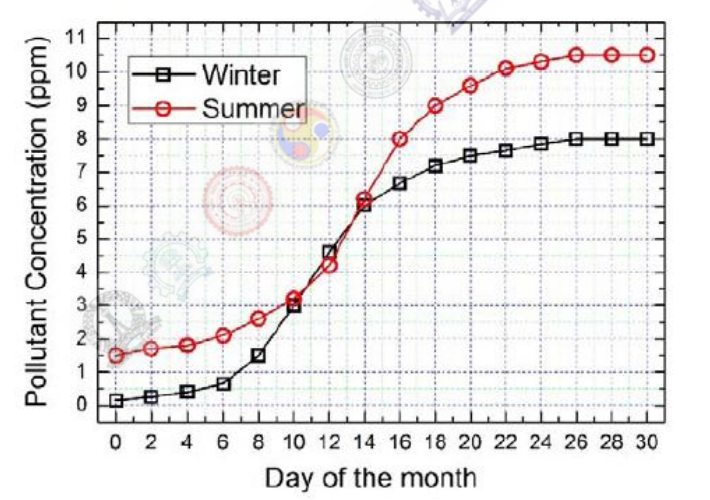
\includegraphics[width=0.5\textwidth]{figures/10.png}
\end{center}

Consider the following statements based on the data shown above:

i. Over the given months, the difference between the maximum and the minimum pollutant concentrations is the same in both winter and summer.  
ii. There are at least four days in the summer month such that the pollutant concentrations on those days are within 1 ppm of the pollutant concentrations on the corresponding days in the winter month.

Which one of the following options is correct?}{10}
\begin{enumerate}
    \item[(A)] Only i
    \item[(B)] Only ii  
    \item[(C)] Both i and ii
    \item[(D)] Neither i nor ii
\end{enumerate}

\vspace{1 cm}

\section*{Technical Section}

% Technical Section
\section*{Technical Section}

\questiona{Matrix  
\[\begin{bmatrix}
0 & 0.5 & 1.5 \\
-0.5 & 0 & 2.5 \\
-1.5 & -2.5 & 0
\end{bmatrix}\]
is a}{1}
\begin{enumerate}
    \item[(A)] Diagonal matrix  
    \item[(B)] Orthogonal matrix  
    \item[(C)] Symmetric matrix
    \item[(D)] Skew-symmetric matrix
\end{enumerate}

\vspace{0.5cm}

\questiona{Direction cosines of the vector $3i - 2j + 6k$ are}{2}
\begin{enumerate}
    \item[(A)] $\left[\frac{3}{7}, -\frac{2}{7}, \frac{6}{7}\right]$
    \item[(B)] $\left[-\frac{3}{7}, \frac{2}{7}, -\frac{6}{7}\right]$  
    \item[(C)] $\left[-\frac{7}{3}, \frac{7}{2}, -\frac{7}{6}\right]$
    \item[(D)] $\left[\frac{7}{3}, -\frac{7}{2}, \frac{7}{6}\right]$
\end{enumerate}

\vspace{0.5cm}

\questiona{Characteristic equation of the matrix  
$\begin{bmatrix}
2 & \sqrt{2} \\
\sqrt{2} & 1
\end{bmatrix}$
with Eigen value $\lambda$ is}{3}
\begin{enumerate}
    \item[(A)] $\lambda^2 + 3\lambda + 4 = 0$
    \item[(B)] $\lambda^2 + 3\lambda - 2 = 0$  
    \item[(C)] $\lambda^2 - 3\lambda = 0$
    \item[(D)] $\lambda^2 + 3\lambda = 0$
\end{enumerate}

\vspace{0.5cm}

\questiona{A box contains three white and four red balls. Two balls are drawn randomly in sequence. If the first draw resulted in a red ball, the probability of getting a second red ball in the next draw is}{4}
\begin{enumerate}
    \item[(A)] 0.33
    \item[(B)] 0.50  
    \item[(C)] 0.67
    \item[(D)] 0.75
\end{enumerate}

\vspace{0.5cm}

\questiona{The probability of getting two heads and two tails from four tosses of the same coin is \_\_\_\_\_.}{5}
\vspace{0.5cm}

\questiona{The purchase price of a tractor is Rs. 5.0 lakh. Considering the constant rate of depreciation as 0.2 in declining balance method, the value of the tractor at the end of $4^\text{th}$ year in lakh will be \_\_\_\_\_.}{6}

\vspace{0.5cm}

\questiona{The pump used in high pressure orchard sprayer is}{7}
\begin{enumerate}
    \item[(A)] Centrifugal pump  
    \item[(B)] Rotary pump  
    \item[(C)] Plunger type positive displacement pump
    \item[(D)] Turbine pump
\end{enumerate}

\vspace{0.5cm}

\questiona{If the Reel Speed Index of a grain combine is more than 1.5, it will increase}{8}
\begin{enumerate}
    \item[(A)] Cutter bar loss
    \item[(B)] Shatter loss  
    \item[(C)] Cylinder loss
    \item[(D)] Straw walker loss
\end{enumerate}

\vspace{0.5cm}

\questiona{A diesel fuel has same ignition delay as that of blend of two reference fuels namely 56\% n-cetane and 44\% hepta-methylnonane. The cetane number of the diesel fuel is \_\_\_\_\_.}{9}

\vspace{0.5cm}

\questiona{Air temperature at the beginning of adiabatic compression in an IC engine is 27°C and the engine compression ratio is 16:1. The temperature of air at the end of the compression in °C will be \_\_\_\_\_.}{10}

\vspace{0.5cm}

\questiona{In fuel property determination, Reid vapour pressure test is used for measuring}{11}
\begin{enumerate}
    \item[(A)] Volatility
    \item[(B)] Viscosity
    \item[(C)] Sulphur content
    \item[(D)] Carbon residue
\end{enumerate}

\vspace{0.5cm}

\questiona{A tractor pulls 8 kN drawbar load against 4 kN rolling resistance. If the tractor develops 57\% tractive efficiency, the slip experienced by the tractor in percentage will be \_\_\_\_\_.}{12}

\vspace{0.5cm}

\questiona{Antecedent Moisture Conditions (AMC) for a soil are defined on the basis of total rainfall occurred during previous \_\_\_\_\_ days.}{13}

\vspace{0.5cm}

\questiona{The seepage analysis in earthen dams is carried out by drawing flownet which consists of equipotential and stream lines. For a homogeneous and isotropic earthen dam, these two lines are always}{14}
\begin{enumerate}
    \item[(A)] orthogonal to each other
    \item[(B)] parallel to each other
    \item[(C)] divergent to each other
    \item[(D)] convergent to each other
\end{enumerate}

\vspace{0.5cm}

\questiona{Remedial measure generally adopted for controlling stream-bank erosion is}{15}
\begin{enumerate}
    \item[(A)] Shelter belts
    \item[(B)] Spurs
    \item[(C)] Brushwood dams
    \item[(D)] Drop spillways
\end{enumerate}

\vspace{0.5cm}

\questiona{Thickness of capillary zone above the water table varies}{16}
\begin{enumerate}
    \item[(A)] linearly with the pore-size of soil
    \item[(B)] inversely with the height of water table
    \item[(C)] linearly with the height of water table
    \item[(D)] inversely with the pore-size of soil
\end{enumerate}

\vspace{0.5cm}

\questiona{A cavity well is a tubewell which has}{17}
\begin{enumerate}
    \item[(A)] gravel pack and a strainer
    \item[(B)] a PVC strainer
    \item[(C)] no strainer
    \item[(D)] a bamboo strainer
\end{enumerate}

\vspace{0.5cm}

\questiona{Modified Hooghoudt's equation for the computation of drain spacing is applicable to}{18}
\begin{enumerate}
    \item[(A)] homogeneous soils
    \item[(B)] anisotropic soils
    \item[(C)] heavy clay soils only
    \item[(D)] layered soils
\end{enumerate}

\vspace{0.5cm}

\questiona{The sum of 'specific yield' and 'specific retention' for an unconsolidated geologic formation is equal to its}{19}
\begin{enumerate}
    \item[(A)] effective porosity
    \item[(B)] total porosity
    \item[(C)] micro-porosity
    \item[(D)] macro-porosity
\end{enumerate}

\vspace{0.5cm}

\questiona{Sphericity of a cube with each side as L is \_\_\_\_\_.}{20}

\vspace{0.5cm}

\questiona{A cylindrical shallow bin is filled with grains having angle of repose of $33^\circ$. The limiting height to diameter ratio of the bin is \_\_\_\_\_.}{21}

\vspace{0.5cm}

\questiona{Length of the husking zone in a rubber roll paddy dehusker, having $d$ as roll diameter, $c$ as clearance between the rolls, and $b$ as grain thickness, is}{22}
\begin{enumerate}
    \item[(A)] $\frac{\pi d}{360} \cos^{-1}\left(\frac{d+c}{d+b}\right)$
    \item[(B)] $\frac{\pi d}{180} \cos^{-1}\left(\frac{d+c}{d+b}\right)$
    \item[(C)] $\frac{\pi d}{360} \sin^{-1}\left(\frac{d+c}{d+b}\right)$
    \item[(D)] $\frac{\pi d}{180} \sin^{-1}\left(\frac{d+c}{d+b}\right)$
\end{enumerate}

\vspace{0.5cm}

\questiona{For a psychrometric ratio of 1003 J kg$^{-1}$ K$^{-1}$, the latent heat of vaporization at the wet bulb temperature of 35°C is 2418.9 kJ kg$^{-1}$. The saturation vapour pressure is 19.7 kPa corresponding to the dry bulb temperature of 60°C. If the relative humidity of air is 20\%, the saturation vapor pressure of the air at the wet bulb temperature in kPa will be \_\_\_\_\_.}{23}

\vspace{0.5cm}

\questiona{A sphere (3.5 cm diameter) made of copper ($\rho = 8954$ kg m$^{-3}$; $C_p = 0.4$ kJ kg$^{-1}$ K$^{-1}$; $k = 375$ W m$^{-1}$ K$^{-1}$) is initially at uniform temperature of 200°C. It is suddenly placed in an environment of 35°C having convective film coefficient of 12 W m$^{-2}$ K$^{-1}$. After 18 minutes of exposure, the temperature of the sphere in °C will be \_\_\_\_\_.}{24}

\vspace{0.5cm}

\questiona{The reaction rate for destruction of \textit{Clostridium botulinum} increases 11 times for temperature rise of 10°C from 121.1°C. The decimal reduction time of this organism is 5.7 s at 121.1°C. The minimum sterilization time in seconds at 135°C, for eight log cycle reduction of the organism, is}{25}
\begin{enumerate}
    \item[(A)] 0.20
    \item[(B)] 0.31
    \item[(C)] 1.63
    \item[(D)] 2.49
\end{enumerate}

\vspace{0.5cm}

\questionb{The areas of seven horizontal cross-sections of a water reservoir at intervals of 9 m are 210, 250, 320, 350, 290, 230 and 170 m$^2$. The estimated volume of the reservoir in m$^3$ using Simpson's rule is \_\_\_\_\_.}{26}

\vspace{0.5cm}

\questionb{Divergence value of a function $(x^2y)\mathbf{i} - (z^3-3x)\mathbf{j} + (4y^2)\mathbf{k}$ at $x = 1$, $y = 2$ and $z = 3$ is \_\_\_\_\_.}{27}

\vspace{0.5cm}

\questionb{Differentiation of $\sqrt{1 + x^2}$ gives}{28}
\begin{enumerate}
    \item[(A)] $\frac{1}{(1 + x^2)}$
    \item[(B)] $\frac{1}{\sqrt{1 + x^2}}$
    \item[(C)] $\frac{\sqrt{1 + x^2}}{x}$
    \item[(D)] $\frac{x}{\sqrt{1 + x^2}}$
\end{enumerate}

\vspace{0.5cm}

\questionb{$I = \int \sqrt{a^2 - x^2} \, dx$ is}{29}
\begin{enumerate}
    \item[(A)] $0.5 \left[ \sqrt{a^2 - x^2} + \sin^{-1}\left(\frac{x}{a}\right) \right]$
    \item[(B)] $0.5 \left[ x\sqrt{a^2 - x^2} + \sin^{-1}\left(\frac{x}{a}\right) \right]$
    \item[(C)] $0.5 \left[ \sqrt{a^2 - x^2} + a^2 \sin^{-1}\left(\frac{x}{a}\right) \right]$
    \item[(D)] $0.5 \left[ x\sqrt{a^2 - x^2} + a^2 \sin^{-1}\left(\frac{x}{a}\right) \right]$
\end{enumerate}

\vspace{0.5cm}

\questionb{A subsolier operating at 400 mm depth requires 15 kW peak drawbar power at 3 km h$^{-1}$ speed. The standard is rigidly fixed vertically on the main frame. The resultant soil resistance acts horizontally at a vertical distance of 450 mm from the main frame. The standard has rectangular cross-section with width to thickness ratio of 4:1, and it fails due to bending. If the allowable bending stress is 90 N mm$^{-2}$, the width of the standard in mm will be \_\_\_\_\_.}{30}

\vspace{0.5cm}

\questionb{A 9-row fluted roller type seed drill with 400 mm ground wheel diameter is used for sowing wheat at 200 mm row spacing. Each fluted roller discharges 6500 mm$^3$ volume of seeds per revolution. The ratio of ground wheel rpm to fluted roller shaft rpm is 2:1. If the bulk density of wheat is 850 kg m$^{-3}$, the seed rate in kg ha$^{-1}$ will be \_\_\_\_\_.}{31}

\vspace{0.5cm}

\questionb{The diameter of feed rollers of a conveyor type power chaff cutter is 100 mm and they are rotating at 90 rpm for cutting the dry fodder. The effective length of each feed roller is 250 mm and the average clearance between them is 15 mm. The compressed density of the material while passing through the feed rollers is 250 kg m$^{-3}$. The throughput capacity of the chaff cutter in ton h$^{-1}$ is \_\_\_\_\_.}{32}

\vspace{0.5cm}

\questionb{The horizontal component of resultant soil thrust (T) acting on each gang of a single acting disc harrow is 1650 N. The resultant downward load (W) acting on each gang is 2500 N. The perpendicular distance of T from the gang axis is 200 mm. In order to get a uniform depth of cut, the distance between the line of action of W and the centre of gang in mm will be \_\_\_\_\_.}{33}

\vspace{0.5cm}

\questionb{A cylindrical parabolic solar collector is designed to heat a fluid that enters the absorber at 140°C at a flow rate of 5 kg min$^{-1}$. The specific heat capacity of the fluid is 1.5 kJ kg$^{-1}$°C$^{-1}$ and its outlet temperature is 180°C. If the incident beam radiation on the plane of aperture is 3000 kJ h$^{-1}$ m$^{-2}$ and useful projected area of the reflector is 2 m × 10 m, the efficiency of the collector in percentage will be \_\_\_\_\_.}{34}

\vspace{0.5cm}

\questionb{A load of 3 kN is acting on a tyre having 150 mm nominal width. The effective friction coefficient of tyre and ground interaction is 0.6 and the kingpin offset is 10 mm. Assuming the tyre impression on ground as circle of diameter same as the tyre nominal width, the kingpin torque of the tyre in N m will be \_\_\_\_\_.}{35}

\vspace{0.5cm}

\questionb{In a tractor power transmission, the input pinion (24 teeth) is in mesh with a gear (46 teeth) on counter shaft and another gear (20 teeth) of counter shaft is in mesh with main shaft gear (50 teeth). The engine is running at 1800 rpm, differential gear ratio is 3.5:1 and final drive ratio is 4:1. If the tractor is fitted with 1.2 m diameter rear wheels, the forward speed of the tractor in km h$^{-1}$ is \_\_\_\_\_.}{36}

\vspace{0.5cm}

\questionb{A hydraulic system comprising of a pump and a single acting cylinder lifts 11 kN load. The pump flow rate is 25 L min$^{-1}$ and its overall efficiency is 80\%. The cylinder diameter is 80 mm and its efficiency is 90\%. If the pressure drop in the hydraulic circuit is 500 kPa, the power required to drive the pump in kW will be \_\_\_\_\_.}{37}

\vspace{0.5cm}

\questionb{A tractor of 19.5 kN weight and 1.8 m wheel base has 70\% static weight on the rear axle. It pulls 8 kN drawbar load parallel to the ground through a hitch point located 450 mm above the ground. The dynamic weight on the rear axle of the tractor under operating condition in kN will be \_\_\_\_\_.}{38}

\vspace{0.5cm}

\questionb{A six-stage centrifugal pump delivers 120 L s$^{-1}$ against a total head of 510 m. If the design speed of this pump is 1450 rpm, the specific speed of the pump will be \_\_\_\_\_.}{39}

\vspace{0.5cm}

\questionb{A watershed of 100 km$^2$ is underlain by an unconfined aquifer having hydraulic conductivity of 15 m day$^{-1}$ and specific yield of 0.20. If 30 million m$^3$ of water is pumped from this aquifer through uniformly distributed wells, the average drop of water table over the watershed in meter will be}{40}
\begin{enumerate}
    \item[(A)] 1.50
    \item[(B)] 0.75
    \item[(C)] 0.06
    \item[(D)] 6.00
\end{enumerate}

\vspace{0.5cm}

\questionb{Match the following items between \textbf{Column-I} and \textbf{Column-II} with the most appropriate combinations:}{41}

\begin{tabularx}{\linewidth}{lXl}
\textbf{Column-I} & & \textbf{Column-II} \\
1) Neutron Probe & & P) Open channel flow \\
2) Pressure Plate Apparatus & & Q) Deep percolation \\
3) Tipping Bucket & & R) Aquifer parameters \\
4) Current Meter & & S) Soil moisture \\
5) Pumping Test & & T) Rainfall intensity \\
6) Lysimeter & & U) Soil-moisture characteristic curve \\
\end{tabularx}

\begin{enumerate}
    \item[(A)] 1-Q, 2-P, 3-T, 4-S, 5-R, 6-U
    \item[(B)] 1-S, 2-U, 3-T, 4-P, 5-R, 6-Q
    \item[(C)] 1-S, 2-R, 3-T, 4-P, 5-Q, 6-U
    \item[(D)] 1-P, 2-U, 3-S, 4-T, 5-R, 6-Q
\end{enumerate}

\vspace{0.5cm}

\questionb{Graded furrows of 80 m length and 0.75 m spacing are used for irrigating a field with an initial furrow stream of 100 L min$^{-1}$. The initial furrow stream flow reaches the lower end of the field in 40 min. Thereafter, the furrow stream flow is reduced to 30 L min$^{-1}$ and the cutback stream flow is continued for 1 hour. The average depth of irrigation over the field in cm will be \_\_\_\_\_.}{42}

\vspace{0.5cm}

\questionb{The soil of a cropped field has field capacity of 25\% and wilting point of 13\% on weight basis. The effective root-zone depth of the crop is 0.70 m and the consumptive use of water by the crop is 5 mm day$^{-1}$. Apparent specific gravity of the soil is 1.50. If the allowable soil moisture depletion is 40\%, the permissible moisture depletion between irrigations and the frequency of irrigation are}{43}
\begin{enumerate}
    \item[(A)] 5 cm; 10 days
    \item[(B)] 10 cm; 7 days
    \item[(C)] 8 cm; 12 days
    \item[(D)] 4 cm; 8 days
\end{enumerate}

\vspace{0.5cm}

\questionb{A watershed of 4.8 km$^2$ generates 4.3 cm runoff from a rain storm of 4-hour duration. The measured rainfall intensities for this storm in successive 30-minute durations are given below:}{44}

\begin{center}
\begin{tabular}{|c|c|c|c|c|c|c|c|c|}
\hline
Time interval (minutes) & 0-30 & 30-60 & 60-90 & 90-120 & 120-150 & 150-180 & 180-210 & 210-240 \\
\hline
Rainfall intensity (cm h$^{-1}$) & 1.6 & 4.8 & 3.2 & 3.4 & 2.2 & 5.0 & 4.2 & 1.2 \\
\hline
\end{tabular}
\end{center}

The value of $\Phi$-index for the watershed in cm h$^{-1}$ will be
\begin{enumerate}
    \item[(A)] 6.5
    \item[(B)] 5.3
    \item[(C)] 2.4
    \item[(D)] 2.1
\end{enumerate}

\vspace{0.5cm}

\questionb{Bunds are to be constructed to conserve rainwater in a farm having 6\% slope. If the horizontal interval between two bunds is 30 m and there is no loss of water, the required height of the bund to store rainwater from an 18 cm rainfall event with 10 years of return period in cm will be \_\_\_\_\_.}{45}

\vspace{0.5cm}

\questionb{A rectangular channel having bed slope of 0.05\% and Manning's roughness coefficient of 0.01 carries a discharge of 5 m$^3$ s$^{-1}$. If the channel is designed as the most economical section, the width of the channel in meter will be \_\_\_\_\_.}{46}

\vspace{0.5cm}

\questionb{A trapezoidal notch, placed over an emergency spillway, has the following details:

\begin{itemize}
\item Top width = 2 m
\item Bottom width = 1 m
\item Height = 0.5 m
\item Coefficient of discharge for the triangular portion = 0.65
\item Coefficient of discharge for the rectangular portion = 0.68
\end{itemize}

For a flow head of 0.4 m over the notch, the discharge in L s$^{-1}$ will be about}{47}
\begin{enumerate}
    \item[(A)] 155
    \item[(B)] 353
    \item[(C)] 508
    \item[(D)] 663
\end{enumerate}

\vspace{0.5cm}

\questionb{In a vertical tube single effect evaporator, the boiling film coefficient inside the tubes is 1350 W m$^{-2}$ K$^{-1}$. Steam condensation film coefficient outside is 7500 W m$^{-2}$ K$^{-1}$. Thermal conductivity of 20 tubes made of SS 304 is 16 W m$^{-1}$ K$^{-1}$. The vertical tubes are 4.3 m long and are of 25 mm ID and 27 mm OD, maintaining a steady 15°C temperature difference across the tube walls. Assume no boiling point rise, no heat losses, the feed enters the evaporator at the boiling point and the latent heat of vaporization of water is 2346.3 kJ kg$^{-1}$. Total water evaporation rate from the evaporator bundle of tubes in kg h$^{-1}$ will be \_\_\_\_\_.}{48}

\vspace{0.5cm}

\questionb{Hot water at 95°C is sent through a countercurrent tube-in-tube heat exchanger with cold water entering at 25°C. Hot/cold water specific heat capacity is 4.2 kJ kg$^{-1}$ K$^{-1}$. Flow rates of hot and cold water are 2.7 and 4.1 kg min$^{-1}$, respectively. Overall heat transfer coefficient is 55 W m$^{-2}$ K$^{-1}$ and the area of heat transfer is 5 m$^2$. Cold water outlet temperature from the heat exchanger in °C will be \_\_\_\_\_.}{49}

\vspace{0.5cm}

\questionb{In a cold storage, 10 metric ton of potato is to be brought down from 30 to 8°C storage temperature in 6 hours of air blast at the evaporator temperature of -10°C. Specific heat capacity of potato is 3.2 kJ kg$^{-1}$ K$^{-1}$. COP of the refrigeration cycle deployed is 4.2 with evaporator load extraction capacity of 210 kJ kg$^{-1}$. Neglecting the respiration load of potato, the refrigerant flow rate and compressor power requirement will be}{50}
\begin{enumerate}
    \item[(A)] 3.9 kg min$^{-1}$; 7.76 kW
    \item[(B)] 9.3 kg min$^{-1}$; 8.50 kW
    \item[(C)] 9.3 kg min$^{-1}$; 7.76 kW
    \item[(D)] 3.9 kg min$^{-1}$; 8.50 kW
\end{enumerate}

\vspace{0.5cm}

\questionb{Steam ($h_f = 632.2$, $h_{fg} = 2113.2$, $h_g = 2745.4$ kJ kg$^{-1}$) at 150°C is used to sterilize milk by direct steam injection. Milk is initially at 90°C and after sterilization, the blend of resultant milk and condensed steam ($h_f = 567.6$, $h_{fg} = 2159.2$, $h_g = 2726.7$ kJ kg$^{-1}$) are at 135°C. Specific heat capacity of milk is 3.8 kJ kg$^{-1}$ K$^{-1}$. Assuming no energy loss, the amount of milk (in kg) sterilized per kg steam supplied is}{51}
\begin{enumerate}
    \item[(A)] 21.57
    \item[(B)] 12.74
    \item[(C)] 9.73
    \item[(D)] 4.48
\end{enumerate}

\vspace{0.5cm}

\questionb{A batch of 1000 kg of apples containing 6.2\% bruised apples is sorted by an electronic colour sorter. The sorted apples contain 927.3 kg red apples and 17.4 kg bruised apples. Remaining red and bruised apples are delivered at the rejection outlet of the sorter. Overall effectiveness of the sorter is \_\_\_\_\_.}{52}

\vspace{0.5cm}

\questionb{Spherical dust particles of 50 µm are settling under gravity in air at 21°C and normal atmospheric pressure. Density of particles is 1250 kg m$^{-3}$ and density of air is 1.2 kg m$^{-3}$. Considering viscosity of air as $1.81 \times 10^{-5}$ Pa s, the settling velocity of dust in mm s$^{-1}$ will be \_\_\_\_\_.}{53}

\vspace{0.5cm}

\questionb{India's annual paddy production is 160 million ton (clean paddy basis). Average husk content of paddy is 22.4\% and milled rice yield is 70\%. Considering 18\% oil content in bran fraction and calorific value of 12 MJ kg$^{-1}$ of husk, the oil potential of bran and energy potential of husk will respectively be}{54}
\begin{enumerate}
    \item[(A)] $2.19 \times 10^6$ ton; $430080 \times 10^{12}$ J
    \item[(B)] $2.19 \times 10^6$ ton; $210450 \times 10^{12}$ J
    \item[(C)] $4.76 \times 10^6$ ton; $210450 \times 10^{12}$ J
    \item[(D)] $4.76 \times 10^6$ ton; $430080 \times 10^{12}$ J
\end{enumerate}

\vspace{0.5cm}

\questionb{A cylindrical silo, 3 m in diameter and 20 m high, is filled with barley having bulk density of 625 kg m$^{-3}$. Coefficient of friction between grain and the bin wall is 0.45 and the ratio of lateral pressure to vertical pressure is 0.4. The lateral pressure at the base of the bin in kPa will be \_\_\_\_\_.}{55}

\vspace{0.5cm}

\vspace{5cm}
\begin{center}
\textbf{END OF THE QUESTION PAPER}
\rule{\textwidth}{0.5pt} 
\end{center}

\end{document}
